\chapter{Formal models for services}
\label{chap:formal}

\lettrine[findent=.2em,lines=2,nindent=0pt]{I}{n} this chapter, we introduce the basic concepts used in the remainder of this thesis. In particular, we introduce \emph{service automata} as a uniform formalism to define the behavior of a service and a service composition. Based on service automata, we define the correctness notions we investigate in the subsequent chapters. We continue by recalling algorithms to construct and characterize correct service automata. We conclude the chapter with a discussion on the choice of service automata as our formal model.





%%%%%%%%%%%%%%%%%%%%%%%%%%%%%%%%%%%%%%%%%%%%%%%%%%%%%%%%%%%%%%%%%%%%%%%%%%%%%%%
\section{Preliminaries}
%%%%%%%%%%%%%%%%%%%%%%%%%%%%%%%%%%%%%%%%%%%%%%%%%%%%%%%%%%%%%%%%%%%%%%%%%%%%%%%

We first recall basic mathematical notions and define several fundamental concepts from computer science.


\paragraph{Sets}
\nomenclature[2M]{$2^M$}{the powerset of $M$}%
\nomenclature[N1]{$\mathds{N}$}{the set of natural numbers (including $0$)}%
\nomenclature[N1+]{$\mathds{N}^+$}{the set of positive natural numbers (excluding $0$)}%

For a set $M$, we denote its cardinality with $|M|$ and its powerset with \smash{$2^M$}. We denote the set of natural numbers (including~$0$) with $\mathds{N}$ and the set of positive natural numbers (excluding~$0$) with~$\mathds{N}^{+}$.


\paragraph{Multisets}
\nomenclature[B]{$\mathcal{B}$}{a multiset}%
\nomenclature[BagsM]{$\Bags(M)$}{the set of all multisets over the set $M$}%
\nomenclature[BagsM]{$\Bags_{k}(M)$}{the set of all $k$-bounded multisets over the set $M$}%
\nomenclature{$\emptymset$}{the empty multiset}%

We denote the set of all multisets over a set $M$ with $\Bags(M)$. We use the list notation for multisets and, for example, write $[x,y,y]$ for the multiset $\{x\mapsto 1, y\mapsto 2, z\mapsto 0\}$ over $\{x,y,z\}$; $\emptymset$ denotes the empty multiset. Addition of multisets $\mathcal{B}_{1},\mathcal{B}_{2}\in\Bags(M)$ is defined pointwise: $(\mathcal{B}_{1}+\mathcal{B}_{2})(x):=\mathcal{B}_{1}(x)+\mathcal{B}_{2}(x)$, for all $x\in M$. For $k\in\mathds{N}$, we denote with $\Bags_{k}(M)$ the set of multisets such that $\mathcal{B}\in\Bags_{k}(M)$ implies $\mathcal{B}(x)\leq k$, for all $x\in M$.


\paragraph{Labeled transition systems}
\nomenclature[q]{$q$}{a state ($q\in Q$)}%
\nomenclature[Q]{$Q$}{a set of states}%
\nomenclature[q0]{$q_{0}$}{the initial state ($q_{0}\in Q$)}%
\nomenclature{$\shortrightarrow$}{a transition relation}%

In this thesis, we distinguish visible (\ie, communicating) and invisible (\ie, internal) actions, yielding an extended definition of labeled transition systems: A \define{labeled transition system} $T=[Q,q_{0},\Sigma,\Sigma^{\tau},{\shortrightarrow}]$ consists of a set of states~$Q$, an initial state~$q_{0}\in Q$, a~set of visible labels~$\Sigma$, a set of \emph{discriminable invisible} labels~$\Sigma^{\tau}$ with $\Sigma\cap\Sigma^{\tau}=\emptyset$, and a~labeled transition relation~${\shortrightarrow}\subseteq Q\times(\Sigma\cup\Sigma^{\tau})\times Q$. For $[q,x,q']\in{\shortrightarrow}$, we shall write~\smash{$q\xrightarrow{x}q'$}. If not clear from the context, we add indices to the constituents of $T$ and refer to its states by $Q_{T}$, for instance.

A state $q'\in Q$ is \define{reachable from a state $q\in Q$}, denoted \smash{$q\xrightarrow{*}q'$}, iff there exists a (possibly empty) sequence of transitions originating in $q$ and ending in $q'$. A state is \define{reachable} iff it is reachable from the initial state~$q_{0}$. If $q$ has no outgoing transitions, we also write $q\not\xrightarrow{}{}$. We define the set $\tau(q)$ of \define{internally reachable states} for a state $q\in Q$ inductively as follows: (base) $q\in \tau(q)$ and (step) if $q'\in \tau(q)$ and \smash{$q'\xrightarrow{x}q''$} with $x\in\Sigma^{\tau}$, then $q''\in \tau(q)$.

For a state $q\in Q$, we define \smash{$\lab(q):=\{x\in\Sigma\mid \exists q'\in Q: q\xrightarrow{x}q'\}$} and $\lab^*(q):=$\break \smash{$\bigcup_{q'\in \tau(q)} \lab(q')$}. A transition system $T$ is \define{complete} iff $\lab(q)=\Sigma$ for each reachable state $q\in Q$. $T$ is \define{deterministic} iff  \smash{$q\xrightarrow{x}q'$} and \smash{$q\xrightarrow{x}q''$} implies $q'=q''$ for each reachable state $q\in Q$. $T$ is \define{$\tau$-free}, if \smash{$q\xrightarrow{x}q'$} implies $x\in\Sigma$ for each reachable state $q\in Q$. $T$ is a \define{finite state} transition system, iff the number of reachable states is finite.

A \define{strongly connected component} (\acronym{SCC}) of $T$ is a maximal set of states $Q'\subseteq Q$ such that $q,q'\in Q'$ implies \smash{$q\xrightarrow{*}q'$}. An \acronym{SCC} $Q'$ is a \define{terminal strongly connected component} iff, for all $q\in Q'$, $q\xrightarrow{*}q'$ implies $q'\in Q'$.


\paragraph{Simulation and structural matching}\label{def:smatching}
\nomenclature[rho]{$\rho$}{a simulation or structural matching relation}%

Let $T$ and $U$ be labeled transition systems. A relation $\varrho\subseteq Q_{T}\times Q_{U}$ is a \define{simulation relation}, iff $[q_{0_{T}},q_{0_{U}}]\in\varrho$ and for all states $q_{T},q'_{T}\in Q_{T}$, all states $q_{U}\in Q_{U}$, and for all labels $x\in\Sigma\cup\Sigma^\tau$ holds: if $[q_{T},q_{U}]\in\varrho$ and \smash{$q_{T}\xrightarrow{x}_{T}q_{T}'$}, then there exists a state $q_{U}'\in Q_{U}$ such that \smash{$q_{U}\xrightarrow{x}_{U}q_{U}'$} and $[q_{T}',q_{U}']\in\varrho$.

We use the distinction between visible and invisible labels to define another relation between states of two transition systems: A relation $\varrho\subseteq Q_{T}\times Q_{U}$ is a \define{structural matching relation}, iff $[q_{0_{T}},q_{0_{U}}]\in\varrho$ and for all states $q_{T},q_{T}'\in Q_{T}$, all states $q_{U}\in Q_{U}$, and for all labels $x\in\Sigma\cup\Sigma^\tau$ holds: if $[q_{T},q_{U}]\in\varrho$ and \smash{$q_{T}\xrightarrow{x}_{T}q_{T}'$}, then (1)~there exists a state $q_{U}'\in Q_{U}$ with \smash{$q_{U}\xrightarrow{x}_{U}q_{U}'$} and $[q_{T}',q_{U}']\in\varrho$ or (2) $x\in\Sigma^{\tau}$ and $[q_{T}',q_{U}]\in\varrho$. The first requirement is the same as for a simulation relation. The second requirement allows the transition system~$T$ to take an arbitrary number of invisible transitions. This makes a structural matching relation similar to a weak simulation relation or a stuttering simulation relation~\cite{BrowneCG_1988_tcs}, but stuttering is only allowed in the labeled transition system $T$.

%%%%%%%%%%%%%%%%%%%%%%%%%%%%%%%%%%%%%%%%%%%%%%%%%%%%%%%%%%%%%%%%%%%%%%%%%%%%%%
\begin{figure}[tb]
\centering
\subfigure[simulation relation]{\makebox[0.49\textwidth]{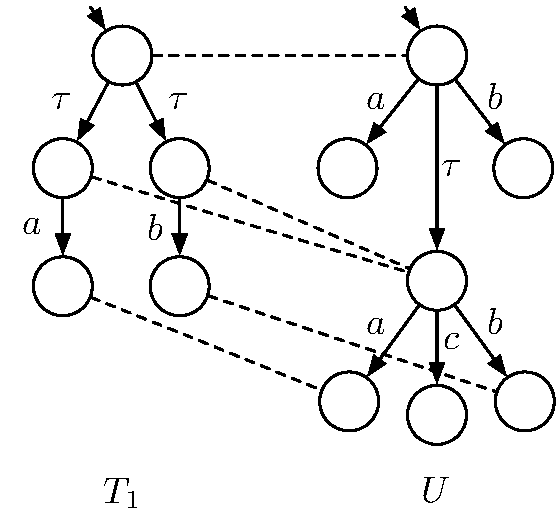
\includegraphics[scale=0.4]{background/simulation}}}\hfill
\subfigure[structural matching relation]{\makebox[0.49\textwidth]{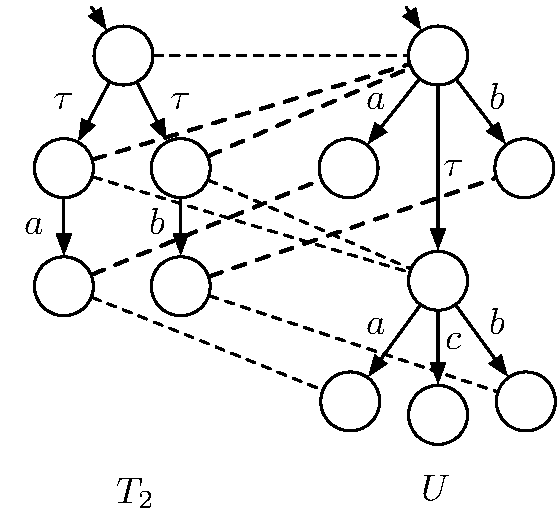
\includegraphics[scale=0.4]{background/matching}}}
\caption{Simulation and structural matching.}
\label{fig:simulationmatching}
\end{figure}
%%%%%%%%%%%%%%%%%%%%%%%%%%%%%%%%%%%%%%%%%%%%%%%%%%%%%%%%%%%%%%%%%%%%%%%%%%%%%%%

A transition system $U$ \define{simulates} (\define{structurally matches}) a transition system $T$ iff there exists a simulation relation (a structural matching relation) $\varrho\subseteq Q_{T}\times Q_{U}$. If the transition systems $T$ and $U$ are not clear from the context, we shall add indices and write $\varrho_{(T,U)}$. \Autoref{fig:simulationmatching} illustrates the simulation and structural matching relation.






%%%%%%%%%%%%%%%%%%%%%%%%%%%%%%%%%%%%%%%%%%%%%%%%%%%%%%%%%%%%%%%%%%%%%%%%%%%%%%%
\section{Modeling services and their composition}
%%%%%%%%%%%%%%%%%%%%%%%%%%%%%%%%%%%%%%%%%%%%%%%%%%%%%%%%%%%%%%%%%%%%%%%%%%%%%%%

%\enlargethispage*{\baselineskip}

In this section, we elaborate the core definitions for services and service compositions. We shall introduce the concept of \emph{ports} to model the (purely syntactic) \emph{interface} of a service. To specify the actual behavior of a service (\ie,~the order in which messages are sent or received), we employ \emph{service automata}.

\medskip

\nomenclature[M-]{$\M$}{the set of all message channels}%
\nomenclature[M-as]{$\M_{s}$}{the set of all synchronous message channels}%
\nomenclature[M-a]{$\M_{a}$}{the set of all asynchronous message channels}%
\nomenclature[E?]{$\E$}{the set of all message events}%
\nomenclature[E?a]{$\send\E$}{the set of all asynchronous send message events}%
\nomenclature[E?b]{$?\E$}{the set of all asynchronous receive message events}%
\nomenclature[E?c]{$\sync\E$}{the set of all synchronous message events}%
\nomenclature[tau]{$\tau$}{a noncommunicating event ($\tau\notin\E$)}%
\nomenclature[M-e]{$\M(e)$}{the message channel of an event $e\in \E$}%
Throughout this thesis, we fix a finite set of message channels $\M$ that is partitioned into asynchronous message channels $\M_{a}$ and synchronous message channels $\M_{s}$. From $\M$, we derive a set of message events $\E$ that is partitioned into asynchronous send events ${!\E}:=\{!m\mid m\in \M_{a}\}$, asynchronous receive events ${?\E}:=\{?m\mid m\in \M_{a}\}$, and synchronous events ${\sync\E}:=\{\sync m\mid m\in \M_{s}\}$. Furthermore, we distinguish a noncommunicating event $\tau\notin \E$. For an event $e\in\{!m, ?m, \sync m\}$, define its message channel as $\M(e):=m$.

In the following definition, we give message channels a direction and group them into \emph{ports} from which we build \emph{interfaces}. An interface lists the ``open'' message channels that are exposed to the environment; that is, to other services. Interfaces can be composed by connecting open message channels. This yields ``closed'' message channels that cannot be used by other services. In this thesis, such closed message channels still belong to the interface. They can be seen as the ``composition history'' of the respective service automaton that implements the interface. This simplifies subsequent definitions and allows for a unified formal model throughout this thesis.

%%%%%%%%%%%%%%%%%%%%%%%%%%%%%%%%%%%%%%%%%%%%%%%%%%%%%%%%%%%%%%%%%%%%%%%%%%%%%%%
\begin{definition}{Port, interface, closed interface}%
\label{def:interface}%
\nomenclature[I]{$I$}{the input message channel of a port $P=[I,O]$}%
\nomenclature[O]{$O$}{the output message channel of a port $P=[I,O]$}%
\nomenclature[Ep]{$\E_{P}$}{the events of a port $P$}%
\nomenclature[M-P]{$\M^{\closed}_{\mathcal{P}}$}{the closed message channels of an interface $\mathcal{P}$}%
\nomenclature[M-P]{$\M^{\open}_{\mathcal{P}}$}{the open message channels of an interface $\mathcal{P}$}%
\nomenclature[EPtau]{$\E^{\tau}_{\mathcal{P}}$}{the internal events of an interface $\mathcal{P}$}%
\nomenclature[EPex]{$\E_{\mathcal{P}}$}{the external events of an interface $\mathcal{P}$}%
%
A pair $P=[I,O]$ is a \define{port} iff $I\cup O\subseteq\M$ and $I\cap O=\emptyset$. $I$ and $O$ are the \define{input message channels} and \define{output message channels} of port $P$, respectively. For $P$, define its events as $\E_{P}:=\{{?m}\mid m\in I\cap \M_{a}\}\cup \{{!m}\mid m\in O\cap \M_{a}\} \cup \,\{{\sync m}\mid m\in (I\cup O)\cap \M_{s}\}$.

Let, for $n\in\mathds{N}$, $\mathcal{P}=\{P_{1},\ldots,P_{n}\}$ be a set of ports with $P_{i}=[I_{i},O_{i}]$ for $i\in\{1,\ldots,n\}$. $\mathcal{P}$ is an \define{interface} iff $I_{i}\cap I_{j}=\emptyset$ for all $i\neq j$ and $O_{i}\cap O_{j}=\emptyset$ for all $i\neq j$. Interface $\mathcal{P}$ is  \define{closed} iff $\bigcup_{i=1}^n I_{i}=\bigcup_{i=1}^n O_{i}$.

From $\mathcal{P}$, derive the set of \define{closed message channels} $\M^{\closed}_{\mathcal{P}}:=(\bigcup_{i=1}^n I_{i})\cap(\bigcup_{i=1}^n O_{i})$, the set of \define{open message channels} $\M^{\open}_{\mathcal{P}}:=(\bigcup_{i=1}^n(I_{i}\cup O_{i}))\setminus\M^{\closed}_{\mathcal{P}}$, the set of \define{internal events} $\E^{\tau}_{\mathcal{P}}:=\{e\in\bigcup_{i=1}^n\E_{P_{i}}\mid \M(e)\in\M^{\closed}_{\mathcal{P}}\}\cup\{\tau\}$, and the set of \define{external events} $\E_{\mathcal{P}}:=\{e\in\bigcup_{i=1}^n\E_{P_{i}}\mid \M(e)\in\M^{\open}_{\mathcal{P}}\}$.
\end{definition}
%%%%%%%%%%%%%%%%%%%%%%%%%%%%%%%%%%%%%%%%%%%%%%%%%%%%%%%%%%%%%%%%%%%%%%%%%%%%%%%

In a port, each message channel has a direction and is either an input message channel or an output message channel. This is natural for asynchronous communication where sending and receiving of messages is decoupled. In contrast, synchronous communication is usually undirected. The classification into input and output is of technical nature and can be compared to the complementary labels $a$ and $\overline{a}$ in \acronym{CCS}~\cite{Milner_1980_ccs}. Nevertheless, the semantics of a message on a finer level of abstraction may induce a natural initiator. For instance, an asynchronous handshake between two parties (\eg,~a pair of a request and an acknowledge message) can be abstracted to an atomic synchronization event.

An interface consists of a set of ports such that communication is bilateral. \emph{A message channel can be used by at most one port as input message channel and by at most one port as output message channel.} If a message channel is used by two ports that way, it is closed and not accessible by other ports any more. This corresponds to \emph{hiding} in process algebra~\cite{Baeten_2005_tcs}. From the message channels of a port and their direction, potential events can be derived. These events can be partitioned into internal events (including~$\tau$) and external events depending on whether the respective message channel is open or closed.

Depending on the context, an interface can be interpreted differently: for a single service, open message channels are exposed to the environment which can invoke the service. An interface with more than one port can be used to model a service orchestrator that interacts with several services simultaneously. In \acronym{WS-BPEL}~\cite{standard_bpel}, the term \emph{partner link} has been coined for such a partition of an interface. Finally, a closed interface describes a choreography of services (cf.~\autoref{chap:realizability}). In this scenario, no message channel is exposed to the environment: the sender and receiver of each message is specified. This \emph{closed world assumption} is common in choreography description languages such as \bpelchor~\cite{DeckerKLW_2007_icws} or \acronym{WS-CDL}~\cite{standard_wscdl}.

Ports and interfaces only describe the syntactic signature of a service consisting of an alphabet of possible events. The behavior itself (\ie,~the order in which messages exchange occurs and when a service terminates) is modeled by \emph{service automata}. A service automaton is a state machine whose transitions are labeled with events derived from a given interface.

%%%%%%%%%%%%%%%%%%%%%%%%%%%%%%%%%%%%%%%%%%%%%%%%%%%%%%%%%%%%%%%%%%%%%%%%%%%%%%%
\begin{definition}{Service automaton}%
\label{def:sa}%
\nomenclature[A]{$A$}{a service automaton}%
\nomenclature[W]{$\Omega$}{a set of final states ($\Omega\subseteq Q$)}%
\nomenclature[P]{$\mathcal{P}$}{an interface}%
A tuple $A=[Q,q_{0},{\shortrightarrow},\Omega,\mathcal{P}]$ is a \define{service automaton} iff
\begin{myitemize}
\item $\mathcal{P}$ is an interface,
\item $[Q,q_{0},\E_{\mathcal{P}},\E_{\mathcal{P}}^{\tau},{\shortrightarrow}]$ is a labeled transition system, and
\item $\Omega\subseteq Q$ is a set of final states.
\end{myitemize}
$A$ is a \define{single-port service automaton}, iff $|\mathcal{P}|=1$; otherwise, $A$ is a \define{multi-port service automaton}. $A$ is \define{closed}, iff $\mathcal{P}$ is a closed interface; otherwise, $A$ is \define{open}.
\end{definition}
%%%%%%%%%%%%%%%%%%%%%%%%%%%%%%%%%%%%%%%%%%%%%%%%%%%%%%%%%%%%%%%%%%%%%%%%%%%%%%%

A service automaton \emph{implements} the ports of its interface by labeling its state transitions with events. If a service automaton implements more than one port, message channels can be closed and the respective events are internal. Whereas internal events can occur independently of the service's environment, external message events can only be realized together with other services. This interplay with other services is defined in terms of the \emph{composition} of service automata.

%%%%%%%%%%%%%%%%%%%%%%%%%%%%%%%%%%%%%%%%%%%%%%%%%%%%%%%%%%%%%%%%%%%%%%%%%%%%%%%
\begin{definition}{Composition of service automata}
\label{def:composition}%
\nomenclature{$\oplus$}{composition of service automata}%
Two service automata $A$ and $B$ are \define{composable} iff $\mathcal{P}_{A}\cap\mathcal{P}_{B}=\emptyset$ and $\mathcal{P}_{A}\cup\mathcal{P}_{B}$ is an interface.

The \define{composition} of two composable service automata $A$ and $B$ is the service automaton $A\oplus B=[Q,q_{0},{\shortrightarrow},\Omega,\mathcal{P}]$ consisting of
\begin{myitemize}
\item $Q:=Q_{A}\times Q_{B}\times \Bags(\M_{a})$,
\item $q_{0}:=[q_{0_{A}},q_{0_{B}}, \emptymset]$,
\item $\Omega:={\Omega_{A}\times \Omega_{B}\times \{\emptymset\}}$,
\item $\mathcal{P}:=\mathcal{P}_{A}\cup\mathcal{P}_{B}$, and
\item ${\shortrightarrow}$ containing exactly the following elements:
\begin{enumerate}
\item for all $m\in\M_{\mathcal{P}_{A}}^{\open} \cap \M_{\mathcal{P}_{B}}^{\open}$ (shared open message channels) and $\mathcal{B}\in\Bags(\M_{a})$,
\begin{myitemize}
\item $[q_{A},q_{B},\mathcal{B}] \xrightarrow{!m} [q_{A}',q_{B},\mathcal{B}+[m]]$, iff $q_{A}\xrightarrow{!m}_{A} q_{A}'$,
\item $[q_{A},q_{B},\mathcal{B}] \xrightarrow{!m} [q_{A},q_{B}',\mathcal{B}+[m]]$, iff $q_{B}\xrightarrow{!m}_{B} q_{B}'$,
\item $[q_{A},q_{B},\mathcal{B}+[m]] \xrightarrow{?m} [q_{A}',q_{B},\mathcal{B}]$, iff $q_{A}\xrightarrow{?m}_{A} q_{A}'$,
\item $[q_{A},q_{B},\mathcal{B}+[m]] \xrightarrow{?m} [q_{A},q_{B}',\mathcal{B}]$, iff  $q_{B}\xrightarrow{?m}_{B} q_{B}'$,
\item $[q_{A},q_{B},\mathcal{B}] \xrightarrow{\sync m} [q_{A}',q_{B}',\mathcal{B}]$, iff $q_{A}\xrightarrow{\sync m}_{A} q_{A}'$ and $q_{B}\xrightarrow{\sync m}_{B} q_{B}'$;
\end{myitemize}
\item for $e\in\E_{\mathcal{P}_{A}}^{\tau}\cup\E_{\mathcal{P}_{B}}^{\tau}$ (internal events) or $e\in\E_{\mathcal{P}}$ (external events) and $\mathcal{B}\in\Bags(\M_{a})$,
\begin{myitemize}
\item $[q_{A},q_{B},\mathcal{B}] \xrightarrow{e} [q_{A}',q_{B},\mathcal{B}]$, iff $q_{A}\xrightarrow{e}_{A} q_{A}'$,
\item $[q_{A},q_{B},\mathcal{B}] \xrightarrow{e} [q_{A},q_{B}',\mathcal{B}]$, iff $q_{B}\xrightarrow{e}_{B} q_{B}'$.
\end{myitemize}
\end{enumerate}
\end{myitemize}
\end{definition}
%%%%%%%%%%%%%%%%%%%%%%%%%%%%%%%%%%%%%%%%%%%%%%%%%%%%%%%%%%%%%%%%%%%%%%%%%%%%%%%

The composability criteria require that the two services must not share a port (\ie,~each port is implemented by exactly one service automaton) and that their union still has the interface property of unidirectional and bilateral communication. Here, keeping closed message channels in the interface is important to keep track of the ``composition history'' of a service.

The composition of two service automata implements the union of their ports. For the state transitions, we distinguish two cases: (1)~communication events between the composed services and (2)~other events that are either internal to one of the composed services or external to the composition. Shared message events do not only influence a service's state, but may also add messages to or remove messages from an asynchronous message channel. To this end, each state of the composition contains a multiset of asynchronously sent messages that have not yet been received and that are pending on the message channel. This represents lossless asynchronous message passing under the assumption that messages can overtake each other. Synchronization between two services does not influence the pending messages. The message buffer is defined to be empty in the initial state and is required to be empty in the final states. The latter requirement rules out interactions that terminate without considering pending messages.

As notational convention, we identify the states of a composition of more than two services by a combination of the participating services' states and a sum of the pending asynchronous messages. For example, we do not identify a state of the composition $(A\oplus B)\oplus C$ with $[ [q_{A},q_{B},\mathcal{B}_{(A\oplus B)}], q_{C}, \mathcal{B}_{(A\oplus B)\oplus C} ]$, but with $[q,\mathcal{B}]$ for $q:=[q_{A},q_{B},q_{C}]$ and $\mathcal{B}:=\mathcal{B}_{A\oplus B}+\mathcal{B}_{(A\oplus B)\oplus C}$. Due to the requirement of bilateral communication and the retainment of closed ports, the composition is\,---\,up to isomorphism\,---\,commutative and associative. Hence, we may treat composition as a partial operation and write $A\oplus B\oplus C$ instead of $(A\oplus B)\oplus C$.


\paragraph{Example.}

As running example for this chapter, consider the service automaton depicted in \autoref{fig:Abuy}. It models a buyer service that receives offers ($o$) from a client and decides whether to accept~($a$) or to reject ($r$) the offer. This decision is modeled by internal $\tau$-steps and is nondeterministic. In case the offer got rejected, the service returns to its initial state ($q_{0}$) and waits for another offer. In case the offer got accepted, the service eventually receives an invoice ($i$) and reaches the final state ($q_{5}$). As it can be seen from the graphical representation, the message channels $a$, $r$, and $i$ are asynchronous, whereas $o$ is a synchronous channel.

\Autoref{fig:Asell} depicts a composable service automaton modeling a seller service. It sends offers until one gets accepted. The composition of the buyer and the seller service yields the closed service automaton in \autoref{fig:composition}. Throughout this thesis, we shall never depict unreachable states.


%%%%%%%%%%%%%%%%%%%%%%%%%%%%%%%%%%%%%%%%%%%%%%%%%%%%%%%%%%%%%%%%%%%%%%%%%%%%%%
\begin{figure}
\centering
\hfill
\subfigure[$A_\text{Buy}$\label{fig:Abuy}]{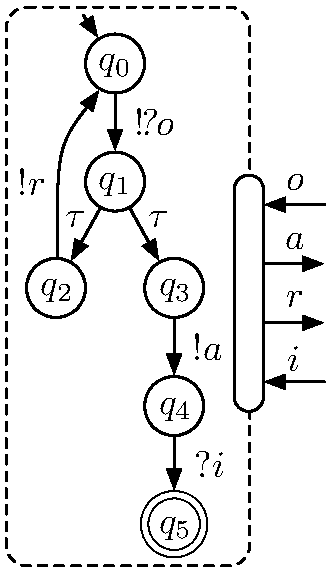
\includegraphics[scale=0.45]{background/running_sa}}\hfill
\subfigure[$A_\text{Sell}$\label{fig:Asell}]{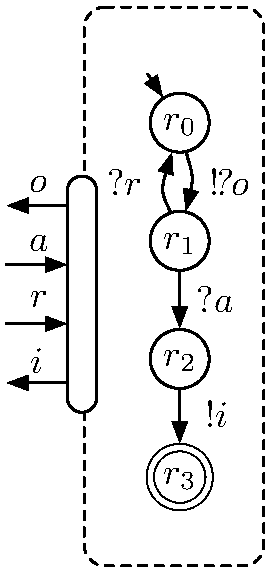
\includegraphics[scale=0.45]{background/running_client}}\hfill
\subfigure[$A_\text{Buy}\oplus A_\text{Sell}$\label{fig:composition}]{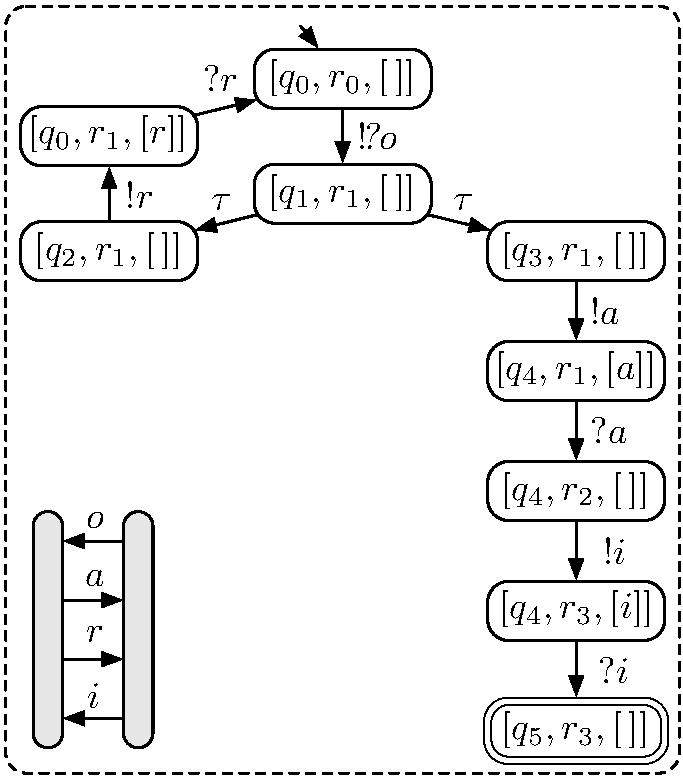
\includegraphics[scale=0.45]{background/running_composition}}\hfill{}
\caption{A buyer service $A_\text{Buy}$ (a) and a seller service $A_\text{Sell}$ (b) modeled as service automata. These automata are composable and (c) depicts their composition $A_\text{Buy}\oplus A_\text{Sell}$.}
\end{figure}
%%%%%%%%%%%%%%%%%%%%%%%%%%%%%%%%%%%%%%%%%%%%%%%%%%%%%%%%%%%%%%%%%%%%%%%%%%%%%%





%%%%%%%%%%%%%%%%%%%%%%%%%%%%%%%%%%%%%%%%%%%%%%%%%%%%%%%%%%%%%%%%%%%%%%%%%%%%%%%
\section{Correctness notions for services}
\label{sect:correctness}
%%%%%%%%%%%%%%%%%%%%%%%%%%%%%%%%%%%%%%%%%%%%%%%%%%%%%%%%%%%%%%%%%%%%%%%%%%%%%%%

Services are not executed in isolation, but are designed to communicate with other services. To this end, reasoning about a service's behavior only makes sense if it is part of a closed composition; that is, all message channels are closed and all events are internal. The behavior of a closed composition can then be defined with the concept of \emph{runs}.

\enlargethispage*{\baselineskip}

%%%%%%%%%%%%%%%%%%%%%%%%%%%%%%%%%%%%%%%%%%%%%%%%%%%%%%%%%%%%%%%%%%%%%%%%%%%%%%%
\begin{definition}{Run, terminating run, deadlocking run}
\label{def:run}%
For a closed service automaton $A=[Q,q_{0},{\shortrightarrow},\Omega,\mathcal{P}]$, a finite or infinite sequence of states $q_{0}q_{1}\cdots$ is a \define{run} of $A$ iff there exists an event $e_{i}$ with \smash{$q_{i}\xrightarrow{e_{i}} q_{i+1}$} for all $i\geq 0$. A~finite run $q_{0}\cdots q_{n}$ is \define{maximal} iff there exists no state $q_{n+1}\in Q$ with \smash{$q_{n}\xrightarrow{*} q_{n+1}$} and $q_{n+1}\neq q_n$. A~maximal run $q_{0}\cdots q_{n}$ \define{terminates} iff $q_{n}\in \Omega$ and \define{deadlocks} iff $q_{n}\notin \Omega$.
\end{definition}
%%%%%%%%%%%%%%%%%%%%%%%%%%%%%%%%%%%%%%%%%%%%%%%%%%%%%%%%%%%%%%%%%%%%%%%%%%%%%%%

With the set of final states we can distinguish desired terminal states, which model the successful completion of a service composition, on the one hand from design errors or undesired deadlocks, on the other hand. We refer to the absence of deadlocks in a composition as \emph{deadlock freedom}. By definition of the composition of service automata, asynchronous message channels must be empty in a final state.

\emph{In this thesis, we do not require every run be extensible to a terminating run} (a property that is usually called \emph{livelock freedom} or \emph{weak termination}). We do allow infinite runs even if no final states are reachable as long as no port is excluded from communication. A service with this property is called \emph{responsive}.

%%%%%%%%%%%%%%%%%%%%%%%%%%%%%%%%%%%%%%%%%%%%%%%%%%%%%%%%%%%%%%%%%%%%%%%%%%%%%%%
\begin{definition}{Responsiveness}
A service automaton $A=[Q,q_{0},{\shortrightarrow},\Omega,\mathcal{P}]$ is \define{responsive} iff for every terminal strongly connected component $Q'$ of $Q$ holds: (1) $Q'\cap\Omega\neq\emptyset$, or (2) for every port $P\in\mathcal{P}$ there exists a state $q\in Q'$ with an outgoing transition that is labeled with an event $e\in\E_{P}$.
\end{definition}
%%%%%%%%%%%%%%%%%%%%%%%%%%%%%%%%%%%%%%%%%%%%%%%%%%%%%%%%%%%%%%%%%%%%%%%%%%%%%%%

If a closed composition of services is responsive, then every infinite run can reach a final state or contains communication events from every port.

As final requirement, communication must not yield an unbounded number of messages pending on asynchronous message channels. The preceded properties are combined in the concept of \emph{compatibility}, which is the core correctness criterion we investigate in this thesis.

%%%%%%%%%%%%%%%%%%%%%%%%%%%%%%%%%%%%%%%%%%%%%%%%%%%%%%%%%%%%%%%%%%%%%%%%%%%%%%%
\begin{definition}{Message bound, \boldmath$k$-compatibility}
\nomenclature[k]{$k$}{a message bound ($k\in\mathds{N}$)}%
\label{def:compatibility}%
Let $A=A_{1}\oplus\cdots\oplus A_{n}$ be a closed service automaton. For a \define{message bound} $k\in\mathds{N}^+$, $A$ is \define{$k$-compatible} iff
\begin{myenumerate}
\item every maximal run of $A$ terminates,
\item $\mathcal{B}(m)\leq k$ for every reachable state $[q,\mathcal{B}]$ of $A$ and $m\in\M_{a}$, and
\item $A$ is responsive.
\end{myenumerate}
\end{definition}
%%%%%%%%%%%%%%%%%%%%%%%%%%%%%%%%%%%%%%%%%%%%%%%%%%%%%%%%%%%%%%%%%%%%%%%%%%%%%%%

A closed composition of services is $k$-compatible iff (1) finite interactions always reach a desired final state in which all message channels are empty, (2) during communication, no asynchronous message channel will ever need to store more than $k$ pending messages, and (3) infinite runs have the possibility to terminate or span all participating ports. A finite and fixed message bound $k$ is motivated by the middleware that realizes the communication of services in reality. The value of $k$ is either known in advance, is derived using capacity considerations or static analysis techniques, or is chosen sufficiently large. In this thesis, we use several models derived from real \acronym{WS-BPEL} processes in which there are hardly any message channels where more than a single pending message made sense. We usually use the term ``compatibility'' without mentioning a specific message bound if the value itself is not of interest or is clear from the context.

Compatibility is a fundamental correctness criterion for closed service compositions. We are aware of more sophisticated criteria, for instance livelock freedom, exclusion of dead activities, or satisfaction of certain temporal logic formulae. Nevertheless, deadlock freedom, bounded communication, and responsiveness would be certainly part of any refined correctness notion. We shall present a refinement of the compatibility notion in \autoref{chap:validation}.

The notion of compatibility can be extended to an open service, yielding the concept of \emph{controllability}.

%%%%%%%%%%%%%%%%%%%%%%%%%%%%%%%%%%%%%%%%%%%%%%%%%%%%%%%%%%%%%%%%%%%%%%%%%%%%%%%
\begin{definition}{\boldmath$k$-controllability, \boldmath$k$-strategy}
\nomenclature[Strat]{$\Strat_{k}(A)$}{the set of all $k$-strategies of a service automaton $A$}%
\label{def:controllability}%
For a message bound $k\in\mathds{N}^+$, a service automaton $A$ is \define{$k$-controllable} iff there exists a service automaton $A'$ such that the composition $A\oplus A'$ is $k$-compatible. We call $A'$ a \define{$k$-strategy} for $A$ and denote the set of all $k$-strategies of $A$ with $\Strat_{k}(A)$.
\end{definition}
%%%%%%%%%%%%%%%%%%%%%%%%%%%%%%%%%%%%%%%%%%%%%%%%%%%%%%%%%%%%%%%%%%%%%%%%%%%%%%%

The term ``strategy'' originates from control theory~\cite{Cassandras99,Ramadge87}: We may see $A'$ as a controller for $A$ imposing compatibility on $A\oplus A'$.

Controllability allows us to reason about a single service while taking its communicational behavior (\ie, the service's local contribution to overall compatibility) into account. It is a fundamental correctness criterion for open services, because a service that cannot interact deadlock freely, bounded, and responsively with \emph{any} other service is certainly ill-designed. In \autoref{chap:diagnosis}, we shall present an algorithm to diagnose the reasons for uncontrollability. From a practical point of view, a $k$-strategy of a service $A$ does not only prove its $k$-controllability, but is also a valuable tool to validate, test, or document the service $A$. Furthermore, a synthesized strategy can be used as a \emph{communication proxy}, which can be implemented (\ie, refined) toward an executable service that is by design compatible to the original service.





%%%%%%%%%%%%%%%%%%%%%%%%%%%%%%%%%%%%%%%%%%%%%%%%%%%%%%%%%%%%%%%%%%%%%%%%%%%%%%%
\section{Construction of strategies}
\label{sect:strategy}
%%%%%%%%%%%%%%%%%%%%%%%%%%%%%%%%%%%%%%%%%%%%%%%%%%%%%%%%%%%%%%%%%%%%%%%%%%%%%%%

In this section, we briefly describe an algorithm from \citet{Wolf_2008_topnoc} to construct a $k$-strategy for service automaton if one exists. The approach is limited to finite state service automata. For infinite state services, a related controllability notion is undecidable~\cite{MassutheSSW_2008_ipl}.

To construct a strategy for a finite state service automaton $A$, we first overapproximate the behavior of \emph{any} service automaton that is composable to $A$. As the internal state of $A$ is not observable, we can only make assumptions based on the messages sent to and received from $A$, respectively. These assumptions and the uncertainty about the exact state can be modeled by a \emph{set} of states the service can assume at a certain point of interaction. These sets of states also include pending asynchronous messages.

%%%%%%%%%%%%%%%%%%%%%%%%%%%%%%%%%%%%%%%%%%%%%%%%%%%%%%%%%%%%%%%%%%%%%%%%%%%%%%%
\begin{definition}{Closure}
\label{def:closure}%
\nomenclature[closure]{$\closure(X)$}{the closure of a set $X$ of states}%
Let $A=[Q,q_{0},{\shortrightarrow},\Omega,\mathcal{P}]$ be a service automaton. For a set $X\subseteq (Q\times \Bags(\M_{A}))$, we define the set $\closure_{A}(X)\subseteq (Q\times \Bags(\M_{a}))$ to be the smallest set satisfying:
\begin{myenumerate}
\item $X\subseteq \closure_{A}(X)$.
\item If $[q,\mathcal{B}]\in \closure_{A}(X)$ and $q\xrightarrow{e}q'$ with $e\in\E^\tau_{\mathcal{P}}$,\\then $[q',\mathcal{B}]\in \closure_{A}(X)$.
\item If $[q,\mathcal{B}]\in \closure_{A}(X)$ and $q\xrightarrow{!m}q'$ with ${!m}\in\E_{\mathcal{P}}$,\\then $[q',\mathcal{B}+[m]]\in \closure_{A}(X)$.
\item If $[q,\mathcal{B}+[m]]\in \closure_{A}(X)$ and $q\xrightarrow{?m}q'$ with ${?m}\in\E_{\mathcal{P}}$,\\then $[q',\mathcal{B}]\in \closure_{A}(X)$.
\end{myenumerate}
\end{definition}
%%%%%%%%%%%%%%%%%%%%%%%%%%%%%%%%%%%%%%%%%%%%%%%%%%%%%%%%%%%%%%%%%%%%%%%%%%%%%%%

The closure of a set of states contains all states that can be reached in~$A$ without requiring any actions of the environment. That is, it contains those states that are reachable by internal events, by receiving already pending asynchronous messages, and by sending asynchronous messages. Synchronous message events are not considered, because synchronization would involve the environment.

Given an open responsive finite state service automaton $A$, the following definition constructs a composable service automaton $\TS^{0}(A)$ that overapproximates the behavior of any service automaton that is composable to $A$. The states of $\TS^{0}(A)$ consist of sets of states of $A$ together with a multiset of pending asynchronous messages. In subsequent steps, those states of $\TS^{0}(A)$ are removed which either violate a given message bound $k$ or deadlock freedom. If the resulting automaton $\TS_{k}(A)$ has a nonempty set of states, $A$ is $k$-controllable and $\TS_{k}(A)$ is a strategy for~$A$.

%%%%%%%%%%%%%%%%%%%%%%%%%%%%%%%%%%%%%%%%%%%%%%%%%%%%%%%%%%%%%%%%%%%%%%%%%%%%%%%
\begin{definition}{Strategy synthesis}
\label{def:synthesis}%
Let $A=[Q_{A},q_{0_{A}},{\shortrightarrow}_{A},\Omega_{A},\mathcal{P}_{A}]$ be an open responsive finite state service automaton with $\mathcal{P}_{A}=\{[I_{1},O_{1}],\ldots,[I_{n},O_{n}]\}$. We define the open service automaton $\TS^{0}(A)=[Q,q_{0},{\shortrightarrow},\Omega,\mathcal{P}]$ with $\mathcal{P}=\{[O,I]\mid [I,O]�\in \mathcal{P}_{A} \cap ( \M_{\mathcal{P}_{A}}^\open\times \M_{\mathcal{P}_{A}}^\open )\}$ and $Q$, $q_{0}$, ${\shortrightarrow}$, and $\Omega$ inductively as follows:
\begin{myitemize}
\item Base: Let $q_{0}:=\closure_{A}(\{[q_{0_{A}},\emptymset]\})$. Then $q_{0}\in Q$.
\item Step: For all $q\in Q$ and $m\in\M$:
\begin{enumerate}
\item If $!m\in \E_{\mathcal{P}}$, let $q':=\closure_{A}(\{ [q_{A},\mathcal{B}+[m]] \mid [q_{A},\mathcal{B}] \in q \})$.\\Then $q'\in Q$ and $q\xrightarrow{!m}q'$.
\item If $?m\in \E_{\mathcal{P}}$, let $q':=\closure_{A}(\{ [q_{A},\mathcal{B}] \mid [q_{A},\mathcal{B}+[m]] \in q \})$.\\ Then $q'\in Q$ and $q\xrightarrow{?m}q'$.
\item If $\sync m\in \E_{\mathcal{P}}$, let $q':=\closure_{A}(\{ [q_{A}',\mathcal{B}] \mid [q_{A},\mathcal{B}] \in q$ $\wedge$ \mbox{$q_{A}\xrightarrow{\sync m}_{A}q_{A}'$}$\})$.\\ Then $q'\in Q$ and $q\xrightarrow{\sync m}q'$.
\end{enumerate}
\item We define $\Omega:=\{ q \in Q�\mid q \cap (\Omega_{A}\times\{\emptymset\}) \neq \emptyset \}$.
\end{myitemize}
For a message bound $k\in\mathds{N}^+$, let \smash{$\TS^{1}_k(A)$} be the service automaton that is obtained from $\TS^{0}(A)$ by removing each state $q\in Q$ that contains a state $[q^*,\mathcal{B}]$ with $\mathcal{B}(m)>k$ for an asynchronous message channel $m\in \M_{a}$.

Given $\TS^{i}_{k}(A)$ ($i\geq 1$), the service automaton $\TS^{i+1}_{k}(A)$ is obtained by removing state $q\in Q_{i}$ if there exists a $[q_{A},\mathcal{B}]\in q$ such that the state~$[q,q_{A},\mathcal{B}]$ of the composition~$\TS_{k}^{i}(A)\oplus A$ is neither final nor has a successor in~$\TS_{k}^{i}(A)\oplus A$. Thereby, the removal of a state includes the removal of its adjacent arcs and all states that become unreachable from the initial state $q_{0}$.

Let $\TS_{k}(A)$ be $\TS^{j}_{k}(A)$ for the smallest $j$ with $\TS_{k}^{j}(A)=\TS_{k}^{j+1}(A)$.
\end{definition}
%%%%%%%%%%%%%%%%%%%%%%%%%%%%%%%%%%%%%%%%%%%%%%%%%%%%%%%%%%%%%%%%%%%%%%%%%%%%%%%

The first overapproximaton $\TS^{0}(A)$ is usually an infinite state service automaton that interacts arbitrarily with $A$. As mentioned earlier, the states $\TS^{0}(A)$ consist of sets of states of the service automaton $A$. If such a state contains a state in which the message bound $k$ is exceeded, it is removed. This yields the finite state service automaton $\TS^{1}_{k}(A)$. In subsequent steps, any deadlocking states are removed until a greatest fixed point, $\TS_{k}(A)$, is reached. The synthesized service automaton is by design responsive, because it does not contain noncommunicating actions.

This algorithm is correct as it was shown by~\citet{Wolf_2008_topnoc}.

%%%%%%%%%%%%%%%%%%%%%%%%%%%%%%%%%%%%%%%%%%%%%%%%%%%%%%%%%%%%%%%%%%%%%%%%%%%%%%%
\begin{proposition}{Synthesis is a strategy~\cite{Wolf_2008_topnoc}}
\label{thm:strategy}%
$A$ is $k$-controllable iff $Q_{\TS_{k}(A)}\neq\emptyset$.
\end{proposition}
%%%%%%%%%%%%%%%%%%%%%%%%%%%%%%%%%%%%%%%%%%%%%%%%%%%%%%%%%%%%%%%%%%%%%%%%%%%%%%%

\citet{Wolf_2008_topnoc} uses a slightly different notion of responsiveness, but the difference does not harm. By definition, $\TS_{k}(A)$ closes all open ports of $A$. \citet{Wolf_2008_topnoc} introduced additional controllability notions that take the partition of message channels over ports into account. We shall introduce these notions in \autoref{chap:realizability} in the context of choreographies.

\paragraph{Example.} \Autoref{fig:mpp} depicts the result of \autoref{def:synthesis} for the buyer service. Due to asynchronous communication, there are two remarkable details:
First, it is also possible to send an invoice message ($i$) in the initial state. This message keeps pending on the message channel until the selling service is able to receive it.
Second, the synthesized strategy also contains an empty state ($q=\emptyset$). This state and its adjacent arcs model behavior that may be present in a strategy, but will be unreachable in the composition with $A$. For instance, a service that not only places an order ($o$), but is also ready to receive an acceptance message ($a$) in the initial state is a valid strategy of the buyer service as long it is also ready to receive $a$ later.

\begin{figure}
\centering
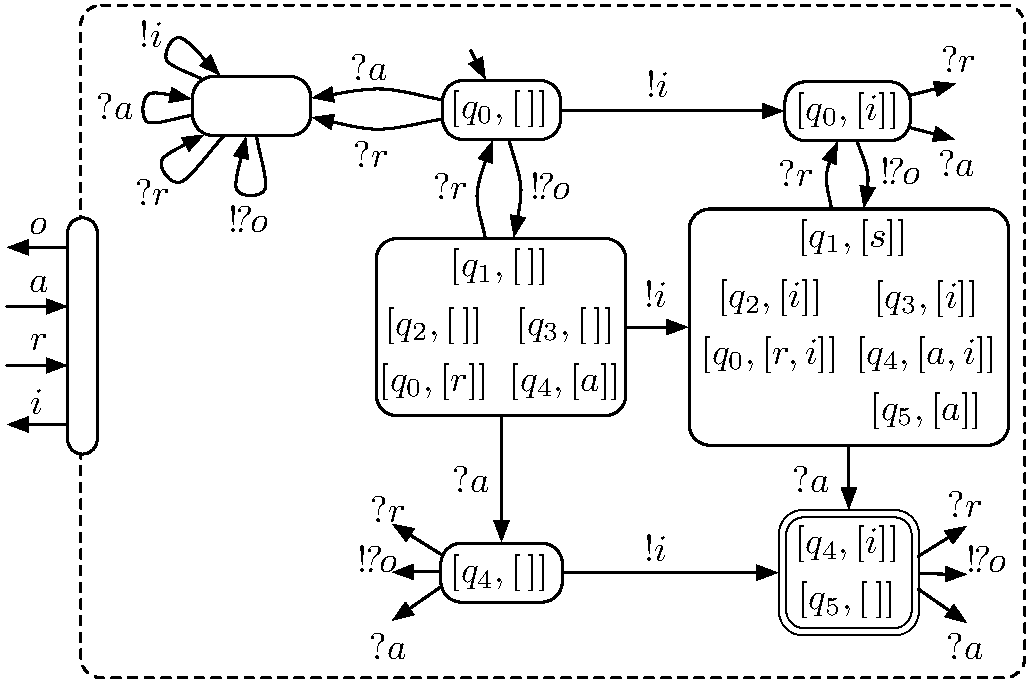
\includegraphics[scale=0.45]{background/running_mpp}
\caption{The synthesized strategy $\TS_{1}(A_\text{Buy})$ of the buyer service $A_\text{Buy}$ from \autoref{fig:Abuy} for $k=1$. Transitions without target states are assumed to have the state $\emptyset\in 2^{Q\times\Bags(\M_{a})}$ as target.}
\label{fig:mpp}
\end{figure}





%%%%%%%%%%%%%%%%%%%%%%%%%%%%%%%%%%%%%%%%%%%%%%%%%%%%%%%%%%%%%%%%%%%%%%%%%%%%%%%
\section{Finite characterization of strategies}
%%%%%%%%%%%%%%%%%%%%%%%%%%%%%%%%%%%%%%%%%%%%%%%%%%%%%%%%%%%%%%%%%%%%%%%%%%%%%%%

In this section, we summarize results from Massuthe and Wolf~\cite{LohmannMW_2007_atpn,Massuthe_2009_phd} to finitely characterize the possibly infinite set of strategies of a service. As a first observation, strategies can be compared with each other with respect to their behavior. In particular, some strategies permit ``more behavior'' than others.

%%%%%%%%%%%%%%%%%%%%%%%%%%%%%%%%%%%%%%%%%%%%%%%%%%%%%%%%%%%%%%%%%%%%%%%%%%%%%%%
\begin{definition}{\boldmath$k$-most-permissive strategy}
\label{def:mps}%
A strategy $B^*\in\Strat_{k}(A)$ of a service automaton $A$ is \define{$k$-most-permissive} iff $B^*$ structurally matches any other $k$-strategy of~$A$.
\end{definition}
%%%%%%%%%%%%%%%%%%%%%%%%%%%%%%%%%%%%%%%%%%%%%%%%%%%%%%%%%%%%%%%%%%%%%%%%%%%%%%%

Thereby, the structural matching relation between service automata is defined on their underlying labeled transition systems. A most-permissive strategy can be seen as a top element in a preorder of service behaviors. This preorder~\cite{Massuthe_2009_phd} is out of scope of this thesis. The strategy synthesized by the algorithm of~\autoref{def:synthesis} is a most-permissive strategy.

%%%%%%%%%%%%%%%%%%%%%%%%%%%%%%%%%%%%%%%%%%%%%%%%%%%%%%%%%%%%%%%%%%%%%%%%%%%%%%%
\begin{proposition}{Synthesis is most-permissive~\cite{Wolf_2008_topnoc}}
Let $A$ be a $k$-controllable service automaton.\\ Then $\TS_{k}(A)$ is a $k$-most-permissive strategy of $A$.\label{prop:mostpermissivestrategy}
\end{proposition}
%%%%%%%%%%%%%%%%%%%%%%%%%%%%%%%%%%%%%%%%%%%%%%%%%%%%%%%%%%%%%%%%%%%%%%%%%%%%%%%

The proof~\cite{LohmannMW_2007_atpn,Wolf_2008_topnoc,Massuthe_2009_phd} is based on \autoref{thm:strategy} and exploits that the composition with any service automaton with ``more'' behavior would not be compatible.

By definition, a $k$-most-permissive strategy $B^*$ of a $k$-controllable service $A$ structurally matches any other $k$-strategy of $A$. The converse does, however, not hold: there exist service automata $C\notin\Strat_{k}(A)$ which are structurally matched by $B^*$. Such services can be ruled out by adding Boolean annotations to the states of a $B^*$.

%%%%%%%%%%%%%%%%%%%%%%%%%%%%%%%%%%%%%%%%%%%%%%%%%%%%%%%%%%%%%%%%%%%%%%%%%%%%%%%
\begin{definition}{Annotated automaton}
\nomenclature[BPhi]{$B^{\varphi}=[B,\varphi]$}{an annotated automaton}%
\nomenclature[final]{$\final$}{proposition that evaluates to true in a final state}%
\nomenclature{$\wedge$}{Boolean conjunction}%
\nomenclature{$\vee$}{Boolean disjunction}%
\nomenclature{$\neg$}{Boolean negation}%
The tuple $B^{\varphi}=[B,\varphi]$ is an \define{annotated automaton} iff $B=[Q,q_{0},{\shortrightarrow},\{P\}]$ is a deterministic $\tau$-free single-port service automaton without final states, and $\varphi$ is an annotation that assigns a Boolean formula to every state $q\in Q$. The formulae are built on $\E_{P}$, an additional proposition $\final$, and the Boolean operators $\wedge$, $\vee$, and $\neg$.
\end{definition}
%%%%%%%%%%%%%%%%%%%%%%%%%%%%%%%%%%%%%%%%%%%%%%%%%%%%%%%%%%%%%%%%%%%%%%%%%%%%%%%

Annotated automata have been introduced by \citet{WombacherFMN_2004_ijwsr} to represent sets of automata. In our context, the Boolean formulae are used to refine the structural matching relation by adding constraints on the edges that leave a state of a service automaton that is structurally matched by a most-permissive partner. Annotated automata have no final states; whether a state of a represented automaton needs to be final is expressed by the proposition $\final$. The truth value of an annotated formula is evaluated by an assignment function.

%%%%%%%%%%%%%%%%%%%%%%%%%%%%%%%%%%%%%%%%%%%%%%%%%%%%%%%%%%%%%%%%%%%%%%%%%%%%%%%
\begin{definition}{Assignment, model}
\nomenclature[b]{$\beta$, $\beta'$}{assignment functions}%
\nomenclature[p]{$\varphi$}{a Boolean formula}%
\label{def:assignment}%
Let $A=[Q,q_{0},{\shortrightarrow},\Omega,\mathcal{P}]$ be a service automaton. We define the \define{assignment} $\beta:Q\times(\E\cup\{\final\})\rightarrow\{\mathit{true},\mathit{false}\}$ as follows:
$$\beta(q,p):=\begin{cases}
\mathit{true}\text{,}&\text{if $p\in \lab^*(q)$,}\\
\mathit{true}\text{,}&\text{if $p=\final$ and $\tau(q)\cap \Omega\neq\emptyset$,}\\
\mathit{false}\text{,}&\text{otherwise}.
\end{cases}$$
A state $q\in Q$ \define{models} a formula $\varphi$ (denoted $q\models\varphi$) iff $\varphi$ evaluates to $\mathit{true}$ under the assignment $\beta(q,\varphi)$. We thereby assume the standard semantics for the Boolean operators $\wedge$, $\vee$, and $\neg$.
\end{definition}
%%%%%%%%%%%%%%%%%%%%%%%%%%%%%%%%%%%%%%%%%%%%%%%%%%%%%%%%%%%%%%%%%%%%%%%%%%%%%%%

An atomic proposition of a formula is true in a state of a service automaton if that state has a respective outgoing edge, possibly reached by a sequence of internal steps. The proposition $\final$ is evaluated to true exactly in final states. The following definition of \emph{matching} combines structural matching and formulae evaluation.

%%%%%%%%%%%%%%%%%%%%%%%%%%%%%%%%%%%%%%%%%%%%%%%%%%%%%%%%%%%%%%%%%%%%%%%%%%%%%%%
\begin{definition}{Matching}\label{def:matching}%
\nomenclature[Match]{$\Match(B^{\varphi})$}{the set of service automata that match with $B^{\varphi}$}%
A service automaton $A$ \define{matches} with an annotated automaton $B^{\varphi}$ iff:
\begin{myenumerate}
\item there exists a structural matching relation $\varrho\subseteq Q_{A}\times Q_{B}$ and
\item for all $[q_{A},q_{B}]\in\varrho$: $q_{A} \models \varphi(q_{B})$.
\end{myenumerate}
Let $\Match(B^{\varphi})$ denote the set of service automata that match with~$B^{\varphi}$.
\end{definition}
%%%%%%%%%%%%%%%%%%%%%%%%%%%%%%%%%%%%%%%%%%%%%%%%%%%%%%%%%%%%%%%%%%%%%%%%%%%%%%%

The first requirement states that a service automaton matches with an annotated automaton only if there exists a structural matching relation. If such a relation exists, it consists of pairs of states for which the formulae must be satisfied in the second step. With this matching predicate, an annotated automaton implicitly defines a (possibly infinite) set of service automata. In particular, we are interested in annotated  automata that exactly characterize the set of $k$-strategies of a service.

%%%%%%%%%%%%%%%%%%%%%%%%%%%%%%%%%%%%%%%%%%%%%%%%%%%%%%%%%%%%%%%%%%%%%%%%%%%%%%%
\begin{definition}{\boldmath$k$-operating guideline}%
\nomenclature[OGkA]{$\OG^k_{A}$}{a $k$-operating guideline of $A$}%
A \define{$k$-operating guideline} for a service automaton $A$ is an annotated automaton\break $\OG^k_{A}=B^\varphi$ such that $\Match(\OG^k_{A})=\Strat_{k}(A)$.
\end{definition}
%%%%%%%%%%%%%%%%%%%%%%%%%%%%%%%%%%%%%%%%%%%%%%%%%%%%%%%%%%%%%%%%%%%%%%%%%%%%%%%

Every $k$-controllable service has a $k$-operating guideline; Masuthe et~al.~\cite{LohmannMW_2007_atpn,Massuthe_2009_phd} provide detailed proofs and a construction algorithm. The core idea is to use a $k$-most-permissive strategy and to annotate each state with a formula that is satisfiable iff those events are present that resolve any deadlock within the associated closure of states while still respecting the message bound.

Beside the aforementioned finiteness, Massuthe and Wolf~\cite{LohmannMW_2007_atpn,Massuthe_2009_phd} further emphasize the following properties that operating guidelines enjoy. These properties are essential for the results we present in subsequent chapters.
\begin{niceitemize}
\item Matching is only defined in terms of structurally matching and formula evaluation. In particular, it does not take the states of the closure (cf.~\autoref{def:closure}) into account. This not only allow for a compact representation (\ie,~only the structure of a most-permissive partner needs to be stored), but also avoids an explicit exposure of the service's internal structure which might be subject to trade secrets.
\item The formulae of an operating guideline can be transformed into positive formulae (\ie,~formulae without negations)~\cite{LohmannW_2009_acsd}. This increases the efficiency of formula evaluation during matching.
\item Having a most-permissive strategy as structure, operating guidelines are operational; that is, $k$-compatible service automata can be easily derived from operating guidelines.
\end{niceitemize}

\medskip

Operating guidelines defined in~\cite{LohmannMW_2007_atpn,Massuthe_2009_phd} base on a compatibility notion that does not include responsiveness. To this end, operating guidelines also characterize services that ``control'' other services by performing an infinite sequence of noncommunicating actions (\eg, $\tau$-loops). Even if the interaction with such unresponsive services is deadlock free and bounded, these services can hardly be used to construct compatible service compositions. Therefore, Defs.~\ref{def:synthesis}--\ref{def:matching} have been adjusted to be applicable in the context of our compatibility criterion.

\paragraph{Example.} \Autoref{fig:og} depicts an operating guideline of the seller service. It has the structure of the most-permissive strategy of \autoref{fig:mpp} and each state is annotated with a Boolean formulae. These formulae constrain the behavior of matching services. For instance, formula ${?a}\wedge{?r}$ demands that a matching service must be able to receive an acceptance~($a$) \emph{and} a rejection ($r$) message. The state modeling unreachable behavior is annotated with \emph{true}: we pose no constraints on unreachable behavior. Note that the events that lead to this \emph{true}-annotated state (\eg, $?a$ and~$?r$ in the initial state) are not mentioned in the formulae.

%%%%%%%%%%%%%%%%%%%%%%%%%%%%%%%%%%%%%%%%%%%%%%%%%%%%%%%%%%%%%%%%%%%%%%%%%%%%%%
\begin{figure}
\centering
\subfigure[$\OG^{1}_{A_\text{Buy}}$\label{fig:og}]{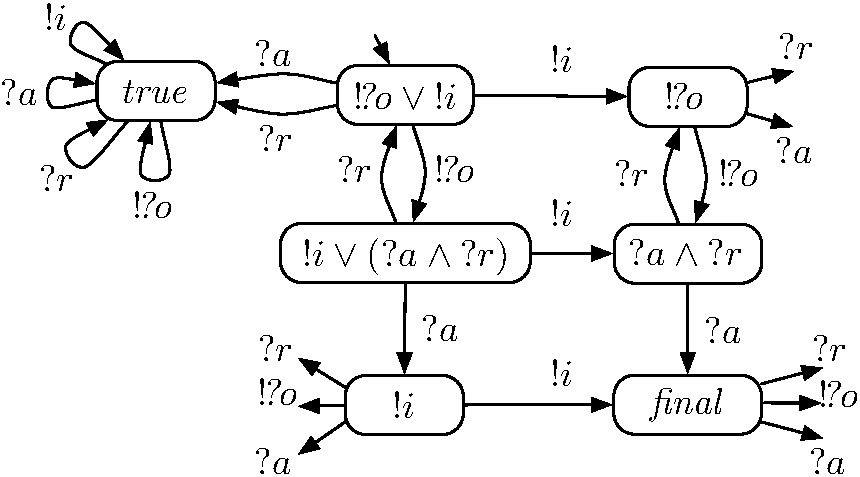
\includegraphics[scale=0.45]{background/running_og}}\hfill
\subfigure[matching with $\OG^{1}_{A_\text{Buy}}$\label{fig:match}]{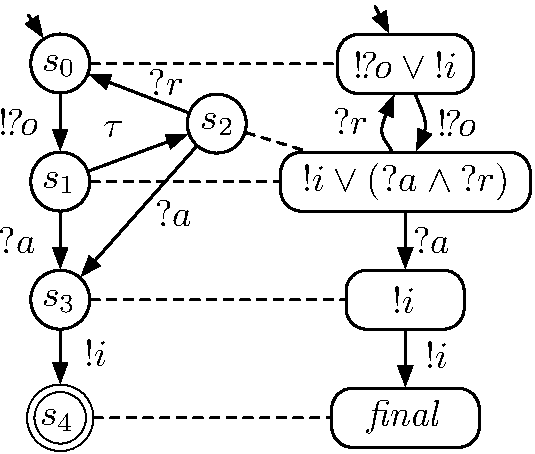
\includegraphics[scale=0.45]{background/running_matching}}
\caption{The operating guideline $\OG^{1}_{A_\text{Buy}}$ (a) of the buyer service $A_\text{Buy}$. Transitions without target states are assumed to have the state with the ``\emph{true}'' annotation as target. A matching service automaton together with the structural matching relation is depicted in (b).}
\end{figure}
%%%%%%%%%%%%%%%%%%%%%%%%%%%%%%%%%%%%%%%%%%%%%%%%%%%%%%%%%%%%%%%%%%%%%%%%%%%%%%

\Autoref{fig:match} depicts an example for a matching service. The dashed lines connect states that are in a structural matching relation between a seller service and a fraction of $\OG^{1}_{A_\text{Buy}}$. The states $s_{1}$ and $s_{2}$ are connected by a $\tau$-annotated edge and match with the same state in the operating guideline. State $s_{1}$ satisfies the formula ${!i}\vee({?a}\wedge{?r})$, because the state $s_{2}$ has both an edge labeled with ${?a}$ and ${?r}$, and this state is internally reachable from $s_{1}$.





%%%%%%%%%%%%%%%%%%%%%%%%%%%%%%%%%%%%%%%%%%%%%%%%%%%%%%%%%%%%%%%%%%%%%%%%%%%%%%%
\section{Experimental Results}\label{sect:background:experiment}
%%%%%%%%%%%%%%%%%%%%%%%%%%%%%%%%%%%%%%%%%%%%%%%%%%%%%%%%%%%%%%%%%%%%%%%%%%%%%%%

Both the strategy synthesis algorithm~\cite{Wolf_2008_topnoc} (cf.\ \autoref{def:synthesis}) and the algorithm to calculate an operating guideline for a service~\cite{LohmannMW_2007_atpn,Massuthe_2009_phd} have been implemented in the tool Wendy~\cite{LohmannW_2009_wendy}. These two algorithms were originally implemented in the tool Fiona~\cite{MassutheW_2008_awpn}. The design goal of Fiona was the combination of several analysis and synthesis algorithms for service behavior. This is reflected by a flexible architecture that aims at the reusability of data structures and algorithms. Although this design facilitated the quick integration and validation of new algorithms, the growing complexity made optimizations more and more complicated.

To overcome these efficiency problems, Wendy is a reimplementation of the two synthesis algorithms as compact single-purpose tool. This reimplementation incorporates the experiments made by analyzing performance bottlenecks through improved data structures and memory management, validation of experimental results which gave a deeper understanding of the parameters of the models that affect scalability, and theoretical observations on regularities of synthesized strategies and operating guidelines.

As a proof of concept, we calculated operating guidelines of several \acronym{WS-BPEL} services from a consulting company. Each process consists around 40 \acronym{WS-BPEL} activities and models communication protocols and business processes of different industrial sectors. To apply the algorithms of this chapter, we first translated the \acronym{WS-BPEL} processes into service automata using the compiler \bpelowfn{}~\cite{Lohmann_2007_hubtr212} implementing the formal semantics we shall discuss in \autoref{chap:verification}.

%%%%%%%%%%%%%%%%%%%%%%%%%%%%%%%%%%%%%%%%%%%%%%%%%%%%%%%%%%%%%%%%%%%%%%%%%%%%%%
\begin{table}
\centering
\caption{Experimental results for strategy synthesis using Wendy.}
\medskip
\label{tab:synthesis}
\footnotesize
\begin{tabular*}{\textwidth}{@{\extracolsep{\fill}}lrrcrrr}
\toprule
& \multicolumn{3}{c}{analyzed service automaton} & \multicolumn{3}{c}{synthesis result} \\ 
service & \multicolumn{1}{c}{$|Q|$} & \multicolumn{1}{c}{$|{\shortrightarrow}|$} & $|\E_{\mathcal{P}}|$ & \multicolumn{1}{c}{$|Q_{\TS}|$} & \multicolumn{1}{c}{$|{\shortrightarrow}_{\TS}|$} & \multicolumn{1}{c}{time (sec)} \\ \midrule
Quotation &            $602$ &      $1{,}141$ & $19$ & $11{,}264$ & $145{,}811$ &   $0$ \\
Deliver goods &       $4{,}148$ & $13{,}832$ & $14$ &  $1{,}376$ &  $13{,}838$ &   $2$ \\ %daniela
{\scriptsize SMTP} protocol &     $8{,}345$ & $34{,}941$ & $12$ & $20{,}818$ & $144{,}940$ &  $29$ \\ %-m3
Car analysis &     $11{,}381$ & $39{,}865$ & $15$ &  $1{,}448$ &  $13{,}863$ &  $49$ \\ %daniela
Identity card &      $14{,}569$ & $71{,}332$  & $11$ &  $1{,}536$ &  $15{,}115$ & $82$ \\
Product order &     $14{,}990$ & $50{,}193$ & $16$ & $57{,}996$ & $691{,}414$ & $294$ \\ %-m2
\bottomrule
\end{tabular*}
\end{table}
%%%%%%%%%%%%%%%%%%%%%%%%%%%%%%%%%%%%%%%%%%%%%%%%%%%%%%%%%%%%%%%%%%%%%%%%%%%%%%

\Autoref{tab:synthesis} lists details on the processes as well as the experimental results. We see that the service automata derived from the \acronym{WS-BPEL} processes have up to 14{,}990 states. These large sizes can be explained by the fact that both the positive as well as the negative control flow (\ie, fault and compensation handling) are modeled. The interfaces consist of up to 19 \acronym{WSDL}~\cite{standard_wsdl} operations.

%%%%%%%%%%%%%%%%%%%%%%%%%%%%%%%%%%%%%%%%%%%%%%%%%%%%%%%%%%%%%%%%%%%%%%%%%%%%%%
\begin{figure}[t!]
\centering
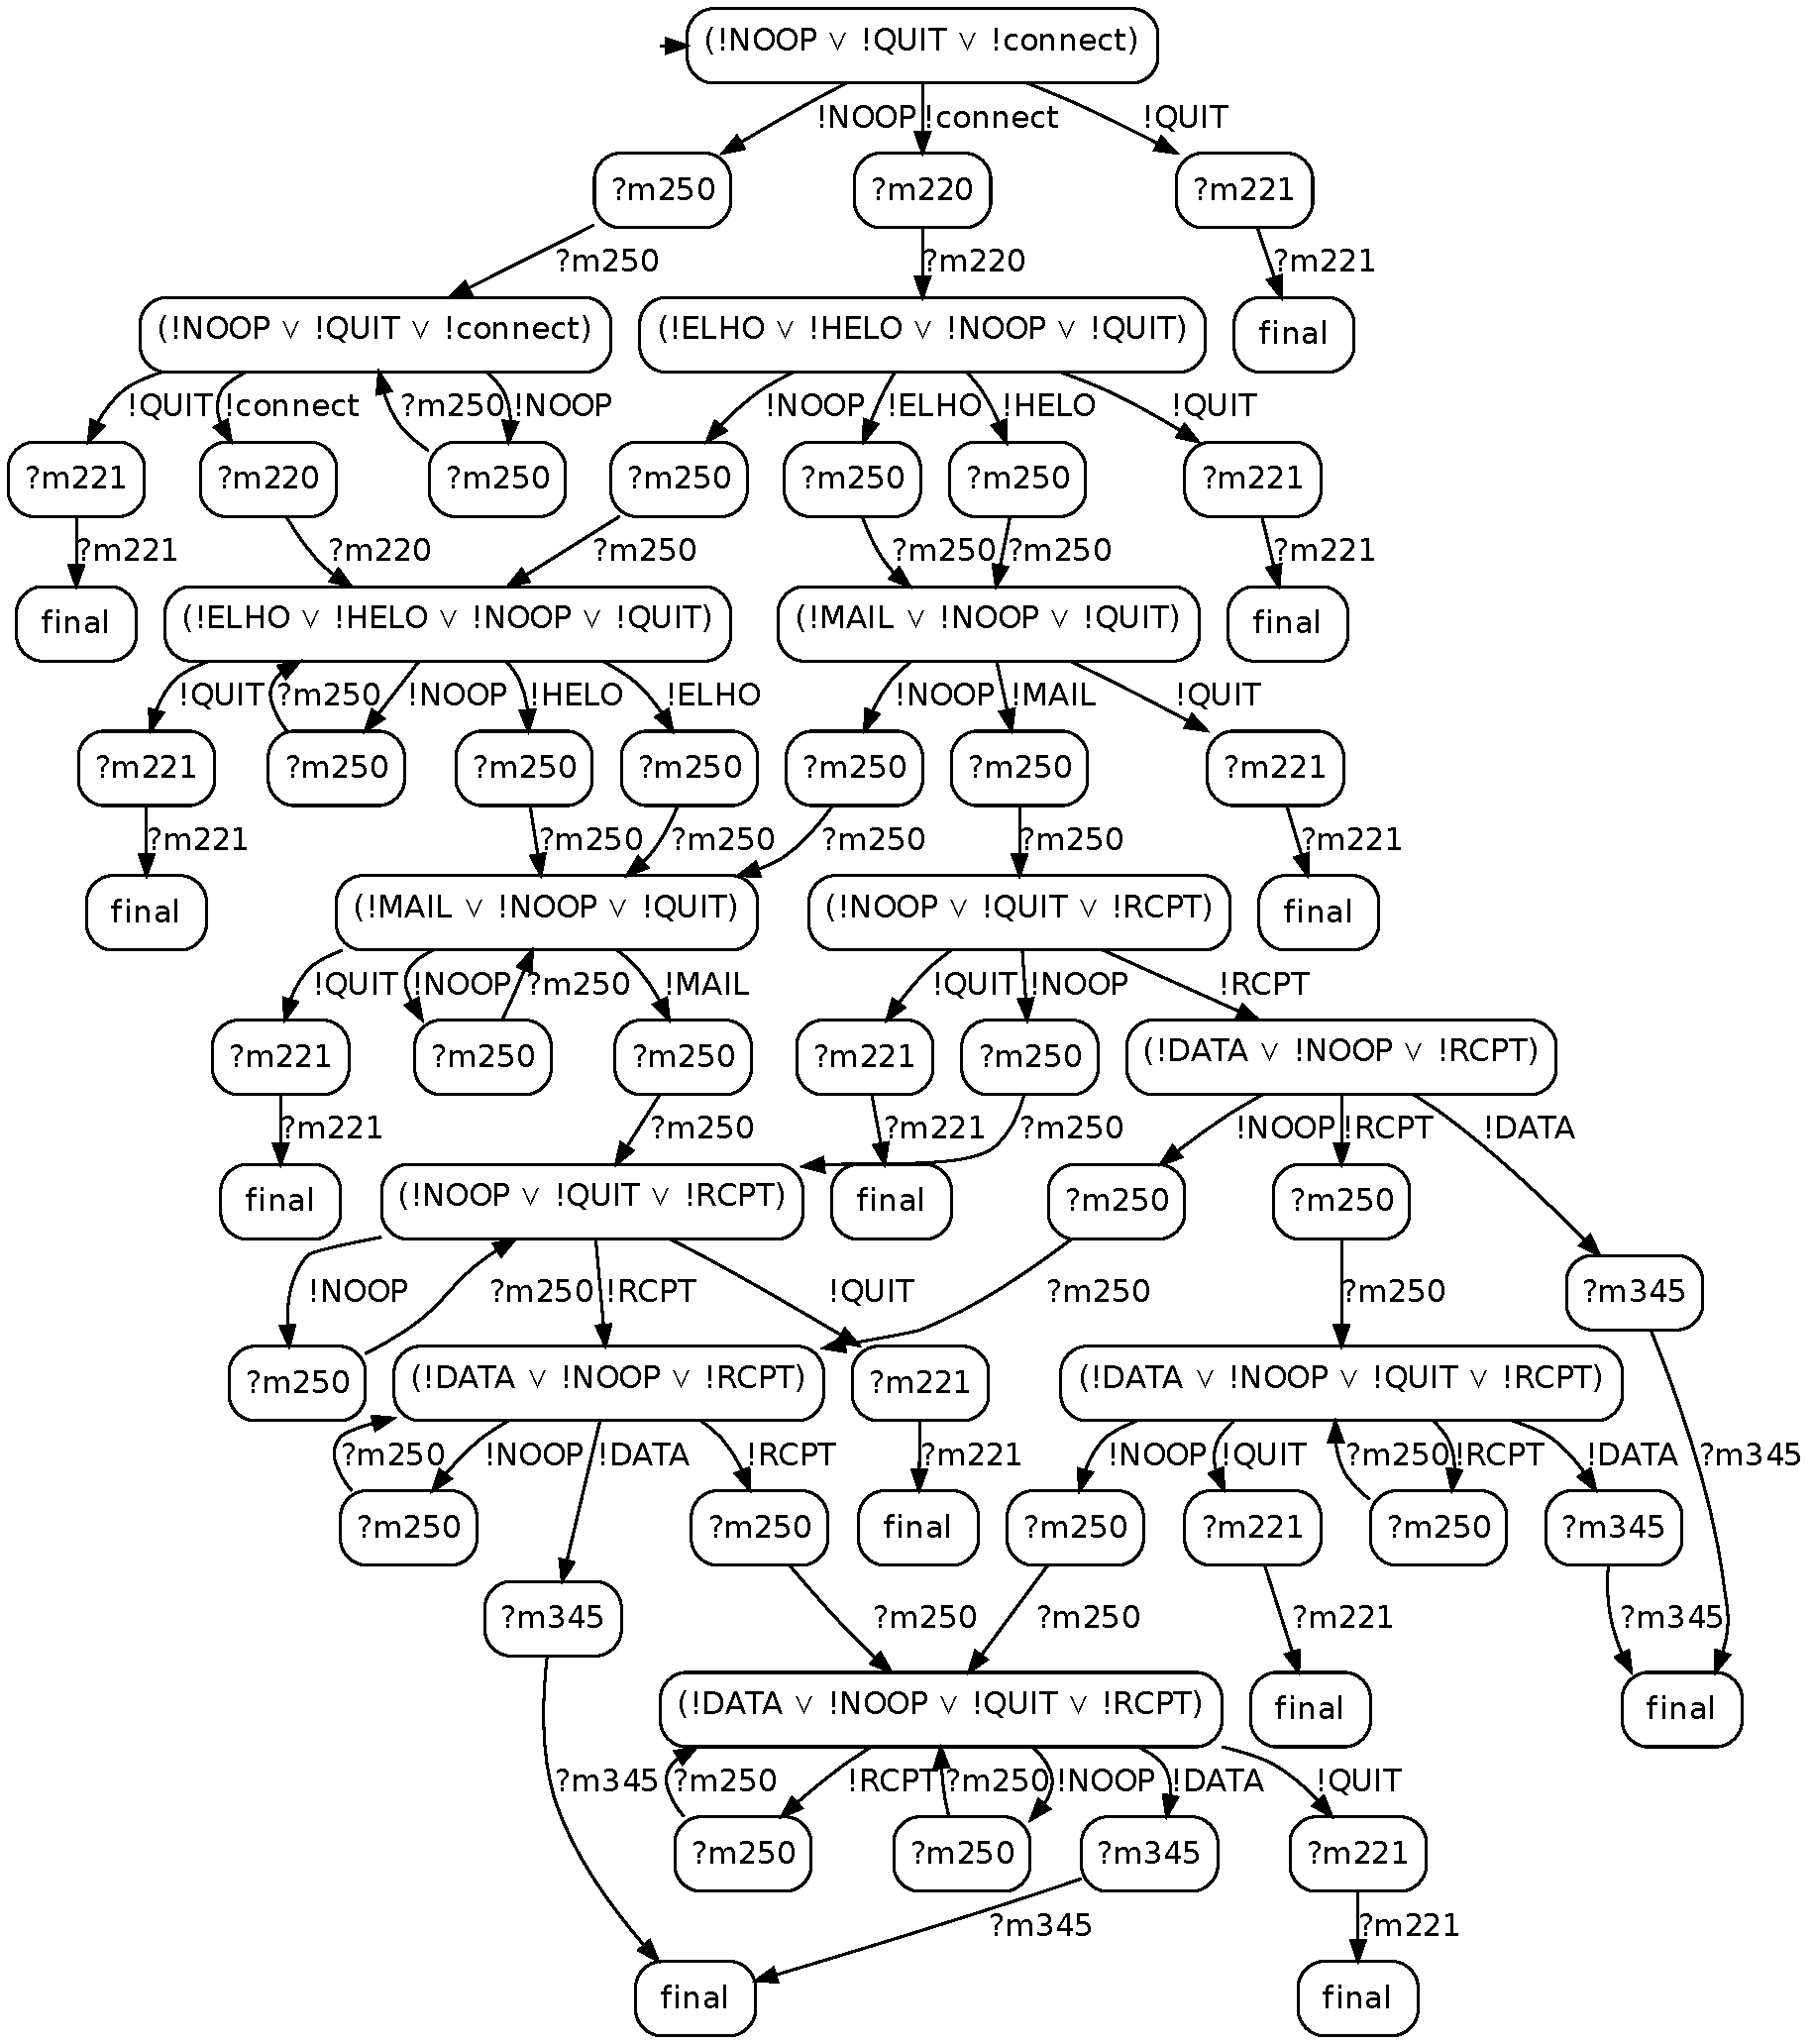
\includegraphics[width=0.9\textwidth]{background/smtp}
\caption{Operating guideline for the \acronym{SMTP} protocol (reduced version) as calculated by the tool Wendy.}\label{fig:smtp}
\end{figure}
%%%%%%%%%%%%%%%%%%%%%%%%%%%%%%%%%%%%%%%%%%%%%%%%%%%%%%%%%%%%%%%%%%%%%%%%%%%%%%


The number of states of the operating guidelines (\ie, the most-permissive strategy) are sometimes much larger than the original service. The number of transitions grows even faster. From these transitions, about the moiety have the empty node $q=\emptyset$ as target state. The analysis takes up to 294 seconds on a 3 \acronym{GH}z computer. This is acceptable, because operating guidelines are usually calculated to be used by the service broker many times. \citet{Massuthe_2009_phd} reports an experiment where the compatibility of two services $A$ and $B$ is verified by model checking the composition $A\oplus B$ on the one hand and calculating the operating guideline $\OG_{A}$ and checking whether $B\in\Match(\OG_{A})$ on the other hand. As result, Massuthe reports that using operating guidelines outperforms model checking in case more than seven checks are made.

In comparison, Fiona could only analyze three of the six services without exceeding 2 \acronym{GB} of memory. For the other models, the analysis was between 5 and 70 times slower than Wendy. To conclude, Wendy allows for the synthesis of strategies and the calculation of operating guidelines of industrial Web services. To give an example of the structure of such strategies, \autoref{fig:smtp} shows an operating guideline of a smaller version of the \acronym{SMTP} protocol.






%%%%%%%%%%%%%%%%%%%%%%%%%%%%%%%%%%%%%%%%%%%%%%%%%%%%%%%%%%%%%%%%%%%%%%%%%%%%%%%
\section{Discussion}
\label{chap:background:discussion}
%%%%%%%%%%%%%%%%%%%%%%%%%%%%%%%%%%%%%%%%%%%%%%%%%%%%%%%%%%%%%%%%%%%%%%%%%%%%%%%

The original contribution of this chapter is the definition of \emph{service automata as a unified formalism to define and reason about services and service compositions that communicate synchronously or asynchronously}. We conclude this chapter with a discussion and a classification of service automata. A discussion of controllability and operating guidelines is beyond the scope of this theses, and we refer the interested reader to the work of Massuthe et al.~\cite{LohmannMW_2007_atpn,Wolf_2008_topnoc,Massuthe_2009_phd}.

\medskip

Communication protocols have been studied and formalized long before the advent of service orientation~\cite{Merlin_1979_ieeesoc,BochmannS_1980_ieeetoc}. Such a formalization must on the one hand specify the protocol or \emph{control flow} itself (\ie,~the order in which messages are exchanged) and the underlying \emph{communication model} (\ie,~the way messages are transfered) on the other hand. Prominent control flow models are finite automata~\cite{HopcroftMU_1979}, Petri nets~\cite{Reisig_1985}, and process algebras~\cite{Baeten_2005_tcs}. As communication model, usually a choice is made between either synchronous or asynchronous message transfer.

We first justify our choice for an automaton-based model for the control flow. This choice is motivated by the correctness criteria that are studied in this thesis: compatibility, controllability, and realizability (cf.~\autoref{chap:realizability}) are \emph{behavioral} criteria defined in terms of states and runs of services and their composition rather than on their structure. Structural approaches, which avoid a state space exploration, are usually defined for special subclasses (\eg,~soundness checks for free-choice Petri nets~\cite{VerbeekBA_2001_tcj}), or allow only for the definition of either necessary \emph{or} sufficient criteria (\eg,~compatibility criteria derived from the state equation~\cite{OaneaW_2009_zeus}). Furthermore, the algorithms to synthesize strategies and operating guidelines are based on states. To this end, we decided to use a formalism with an explicit notion of states rather than models with an implicit notion of states, such as Petri nets or process algebras. This decision also takes into account that none of the algorithms presented in this thesis currently exploits the ability of Petri nets and process algebras to explicitly express concurrency. Nevertheless, Petri~nets can be later used to compactly represent service automata and operating guidelines~\cite{LohmannW_2009_acsd}.

Service automata are introduced as a uniform instrument to \emph{reason} about correctness of services rather than to \emph{model} services. To create models of services, domain-specific languages, such as \acronym{BPMN} or \acronym{WS-BPEL}, and graphical formalisms, such as Petri nets or \acronym{MSC}s, are far more accessible to domain experts. Such models can, however, be easily translated into service automata:  \citet{Massuthe_2009_phd} presents a bidirectional translation between open nets and service automata, and there exists a variety of translations~\cite{BreugelK2006,LohmannVOSA_2009_ijbpim,LohmannVD_2008_topnoc} of service description languages into Petri nets and other formalisms related to automata.

\citet{KazhamiakinPS_2006_www} compare the expressiveness of different communication models with respect to their ability to detect errors in service compositions. They define a parametrized \emph{state transition system with channels}. Depending on the parameters on numbers, sizes, and ordering abilities of the channels, they constitute a hierarchy of communication models and discuss the tradeoff between expressiveness and analysis performance.

The most restricted communication model is synchronous communication. It allows for simple models and efficient verification, but makes strong assumptions on the underlying infrastructure implementing the message exchange between the services. In particular, the whole message transfer is considered to be instantaneous. Formalisms using synchronous communications include service automata, \emph{I/O automata}~\cite{Lynch_1996}, \emph{interface automata}~\cite{AlfaroH_2001_fse}, the ``Roman Model''~\cite{BerardiCGLM_2003_icsoc}, and \emph{message exchanging finite state automata}~\cite{BaldoniBMP_2006_icsoc}. Synchronous communication is also  common in interaction models, for instance \emph{interaction Petri nets}~\cite{DeckerW_2007_bpm}. \citet{Wolf_2007_sa} and \citet{Wolf_2008_topnoc} study Petri net models in which multiple synchronous events may occur simultaneously. This extension has an impact on compatibility and controllability, because a set of simultaneously occurring synchronous events can reach different states than an arbitrary interleaving of these events. Due to increased verification complexity and little practical relevance, we decided not to extend our communication model this way.

A more general communication model decouples the sending and the receiving of a message, but still assumes that the order of sending messages implies an order in which these messages are received; that is, messages are not reordered during communication. This is typically modeled by \acronym{FIFO} queues. Decidability issues in the context of unbounded queues were studied with \emph{communicating finite state machines}~\cite{BrandZ_1983_jacm}, and recent work employing \acronym{FIFO} queues usually assume a finite bound~\cite{FuBS_2004_www,FuBS_2005_tse}, sometimes even fixed to the size of one~\cite{BalbianiCF_2008_ieeeservice,BerardiCGHM_2005_vldb}.

Finally, the most general communication model assumes unordered message buffers which can be modeled using multisets. Beside service automata, \emph{concurrent automata}~\cite{AlurEY_2003_tse} and \emph{open nets}~\cite{KindlerMR_2000_bpm,Kindler_1997_atpn,Martens_2003_phd,ReisigSS_2005_ife,MassutheRS_2005_amct} follow this approach in which no assumptions are made about the infrastructure other than messages not to get lost.

\citet{BultanFHS_2003_www} stress that the verification of asynchronous communication is more complex than synchronous communication. To this end, \citet{FuBS_2005_tse} examine under which conditions asynchronous communication can be safely abstracted to synchronous communication. They provide sufficient conditions which include the strong requirement that at most one message event is activated in every reachable state of a composition. We investigated the impact of communication models to controllability~\cite{Lohmann_2010_zeus} and showed that small variations in the communication model (\eg, changing the message bound) can make controllable services uncontrollable, and vice versa.

\medskip

To conclude, service automata support \emph{both} synchronous and (unordered) asynchronous communication and hence cover the entire range of the communication model hierarchy~\cite{KazhamiakinPS_2006_www}. The ability to mix synchronous and asynchronous communication (similar to \cite{Wolf_2007_sa,BultanF_2008_soca,Wolf_2008_topnoc}) allows us to faithfully represent and reason about service models at different levels of abstraction.
